\section*{Introduction}


This report\footnote{This is the arxiv.org version of this tutorial.
  Some graphics have been compressed to respect arxiv.org's 10MB limit on paper size,
  and do not reflect the full image quality.
}
summarizes the content of the NIPS 2016 tutorial on {\em generative adversarial networks}
(GANs) \citep{Goodfellow-et-al-NIPS2014-small}.
The tutorial was designed primarily to ensure that it answered most of
the questions asked by audience members ahead of time, in order to make sure
that the tutorial would be as useful as possible to the audience.
This tutorial is not intended to be a comprehensive review of the field
of GANs; many excellent papers are not described here, simply because
they were not relevant to answering the most frequent questions, and because
the tutorial was delivered as a two hour oral presentation and did not
have unlimited time cover all subjects.

The tutorial describes:
(1) Why generative modeling is a topic worth studying,
(2) how generative models work, and how GANs compare to other generative models,
(3) the details of how GANs work,
(4) research frontiers in GANs, and
(5) state-of-the-art image models that combine GANs with other methods.
Finally, the tutorial contains three exercises for readers to complete,
and the solutions to these exercises.

The slides for the tutorial are available in PDF and Keynote format at the following URLs:

\url{http://www.iangoodfellow.com/slides/2016-12-04-NIPS.pdf}

\url{http://www.iangoodfellow.com/slides/2016-12-04-NIPS.key}

The video was recorded by the NIPS foundation and should be made available at a later date.

Generative adversarial networks are an example of {\em generative models}.
The term ``generative model'' is used in many different ways.
In this tutorial, the term refers to any model that takes a training set,
consisting of samples drawn from a distribution $\pdata$, and learns to
represent an estimate of that distribution somehow.
The result is a probability distribution $\pmodel$.
In some cases, the model estimates $\pmodel$ explicitly, as shown in
\figref{fig:density}.
In other cases, the model is only able to generate samples from
$\pmodel$, as shown in \figref{fig:generative_machine}.
Some models are able to do both.
GANs focus primarily on sample generation, though it is possible to
design GANs that can do both.

\begin{figure}
\center
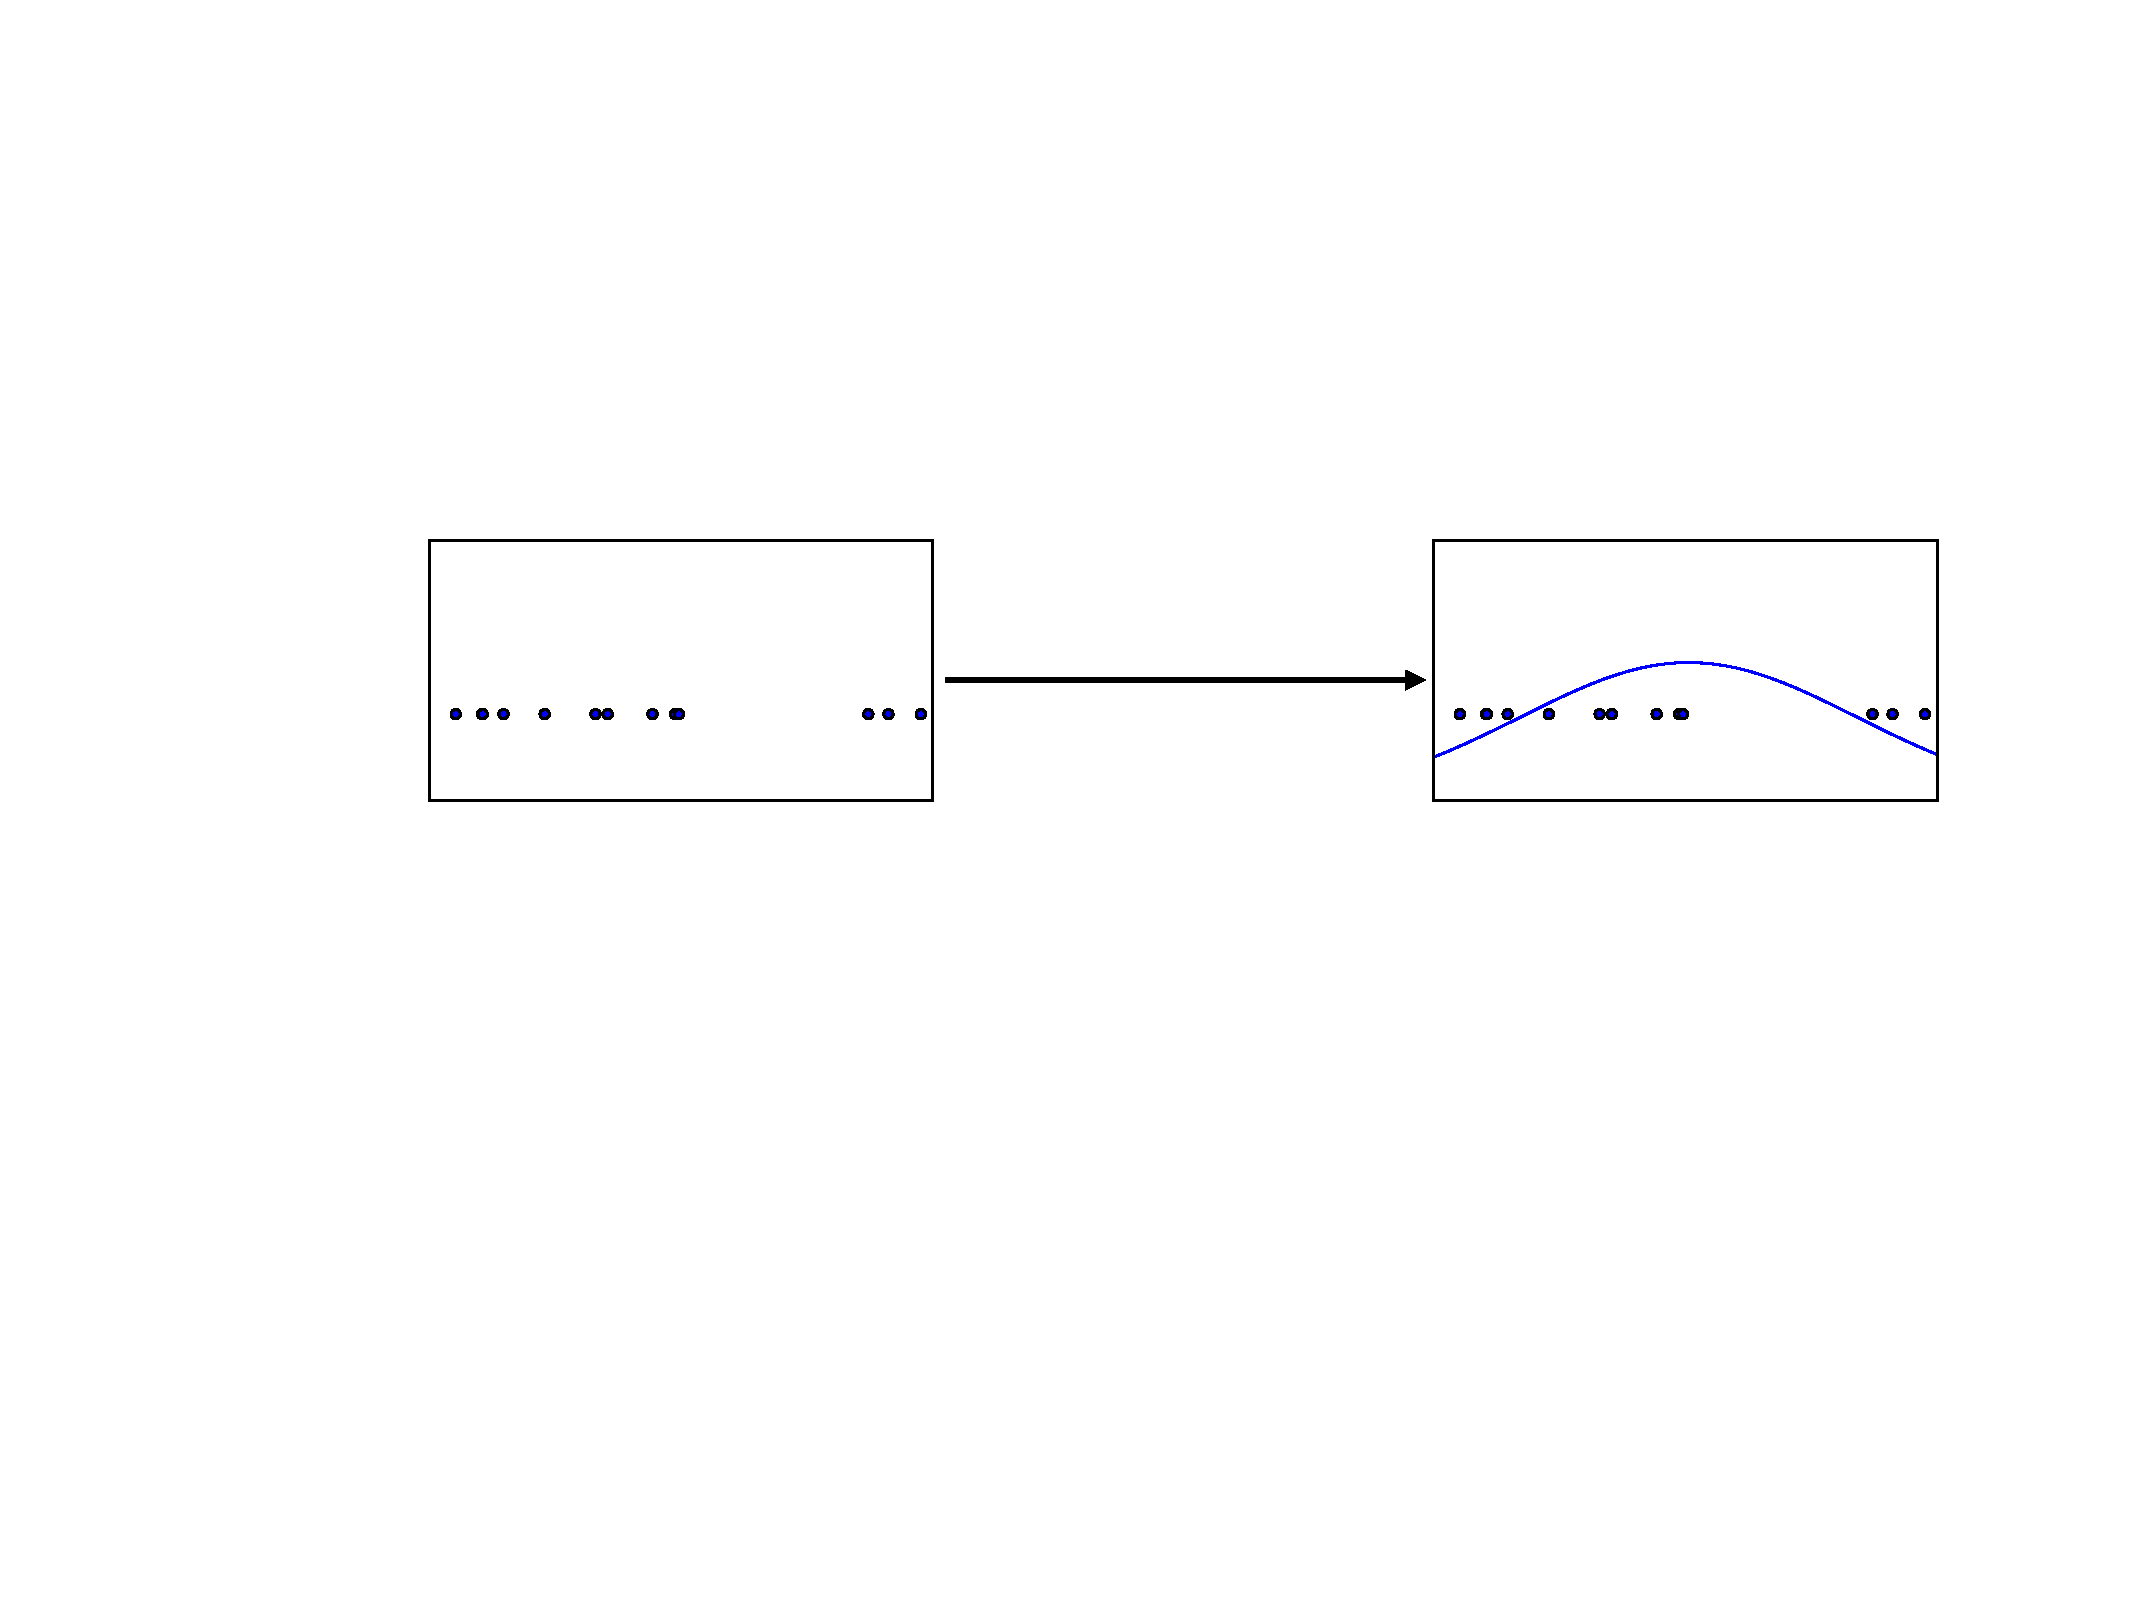
\includegraphics[width=\textwidth]{density}
\caption{Some generative models perform density estimation.
These models take a training set of examples drawn from an unknown
data-generating distribution $\pdata$ and return an estimate of that
distribution. The estimate $\pmodel$ can be evaluated for a particular
value of $\vx$ to obtain an estimate $\pmodel(\vx)$ of the true
density $\pmodel(\vx)$.
This figure illustrates the process for a collection of samples of
one-dimensional data and a Gaussian model.
}
\label{fig:density}
\end{figure}

\begin{figure}
  \center
  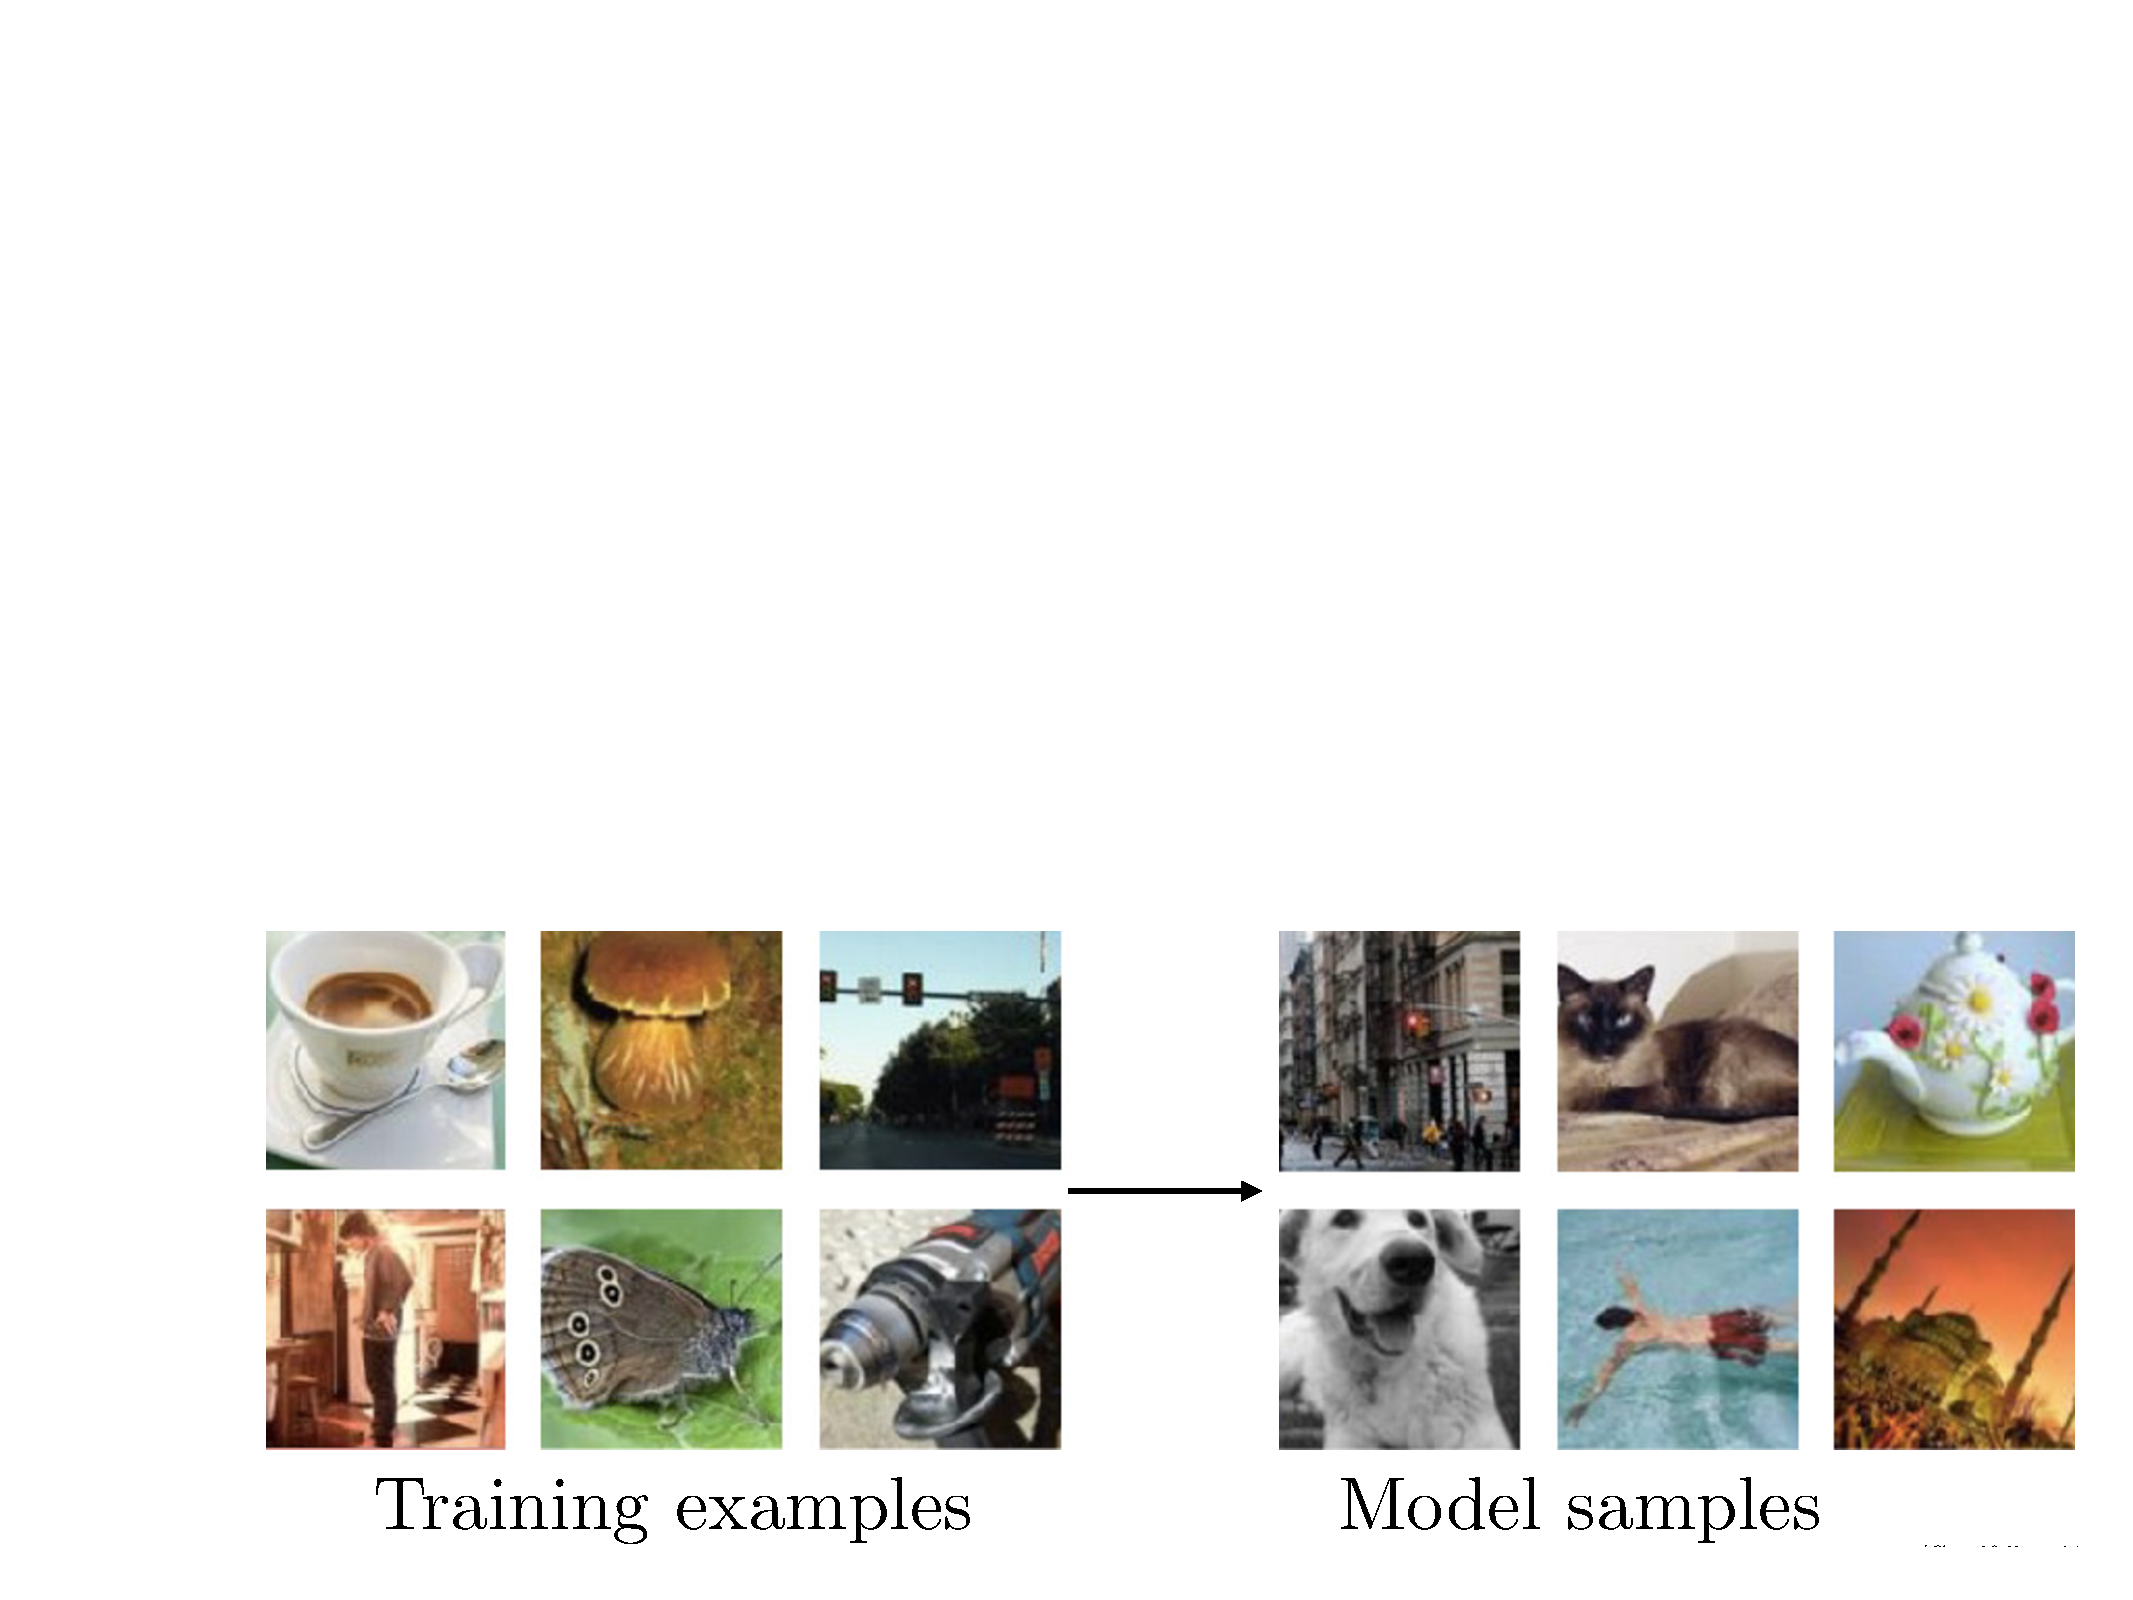
\includegraphics[width=\textwidth]{generative_machine.pdf}
  \caption{Some generative models are able to generate samples
    from the model distribution.
    In this illustration of the process, we show samples from
    the ImageNet \citep{imagenet_cvpr09,Deng2010,ILSVRCarxiv14} 
    dataset.
    An ideal generative model would be able to train on examples
    as shown on the left and then create more examples from the
    same distribution as shown on the right.
    At present, generative models are not yet advanced enough to
    do this correctly for ImageNet, so for demonstration purposes
    this figure uses actual ImageNet data to illustrate what an
    ideal generative model would produce.
  }
  \label{fig:generative_machine}
\end{figure}

